% % % Set the style for this file:
\pagestyle{standard}

% % % Beginning of the chapter
\chapter{Experimental setup}\label{chapter2}

	% % % Set the style for the first page:
	\thispagestyle{chapter-first-page}
	
	\section{Custom Thermal Chamber.}\label{section2.1}
	
		For the infrared measurements, the thermomechanical petal prototype was placed inside a customised thermal chamber where, on one extreme, the Petal is installed in its support (Figure 2.1 left) and on the opposite extreme the IR camera is mounted in a mobile platform that can move in X and Y coordinates thanks to an Arduino controlled Gantry System (Figure 2.1 right). Temperature and relative humidity (RH) inside the chamber can be monitored using three SHT21 sensors coupled to a Raspberry Pi.
		
		\begin{figure}[ht!]
			\centering
			\captionsetup{justification=centering,margin=2cm}
			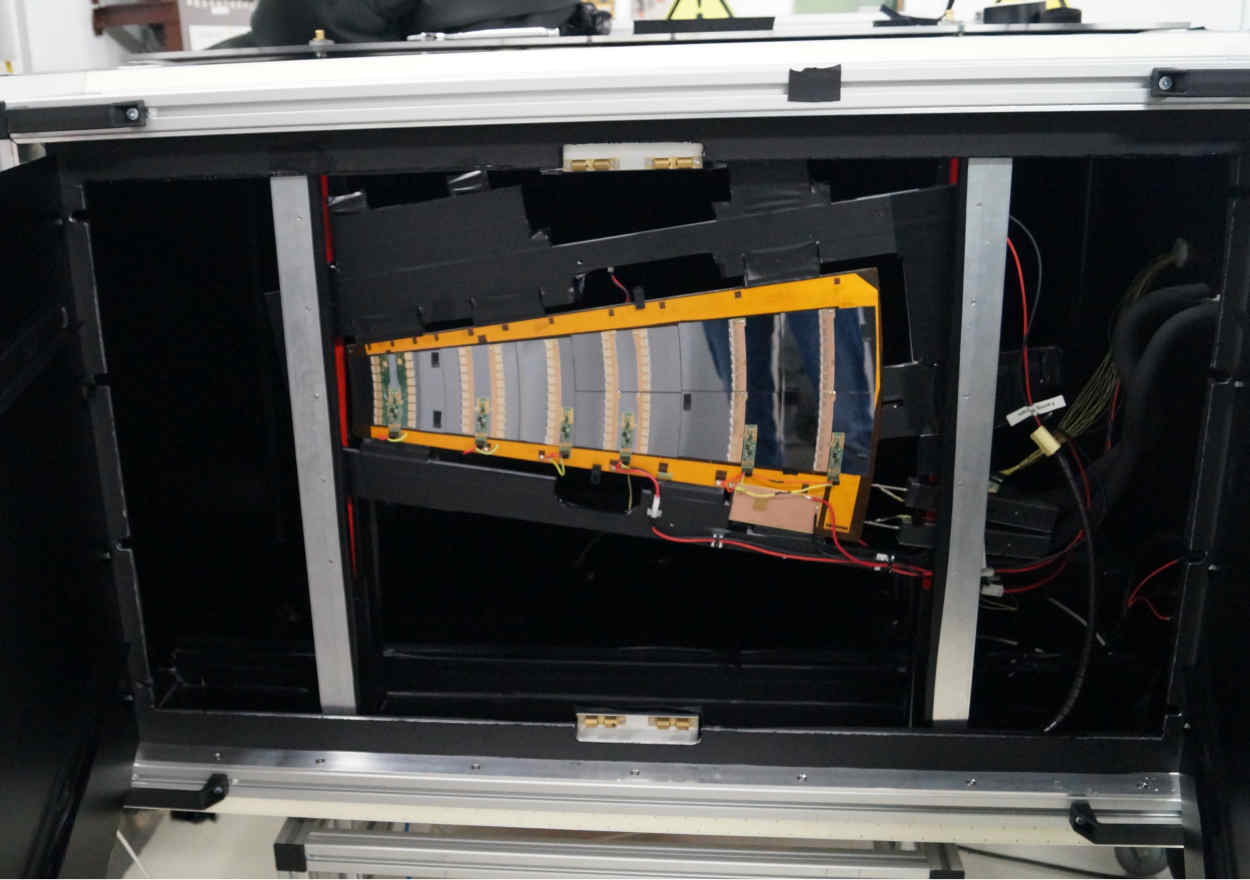
\includegraphics[scale=0.25]{Figures/Chapter02/ChamberBack.pdf}
			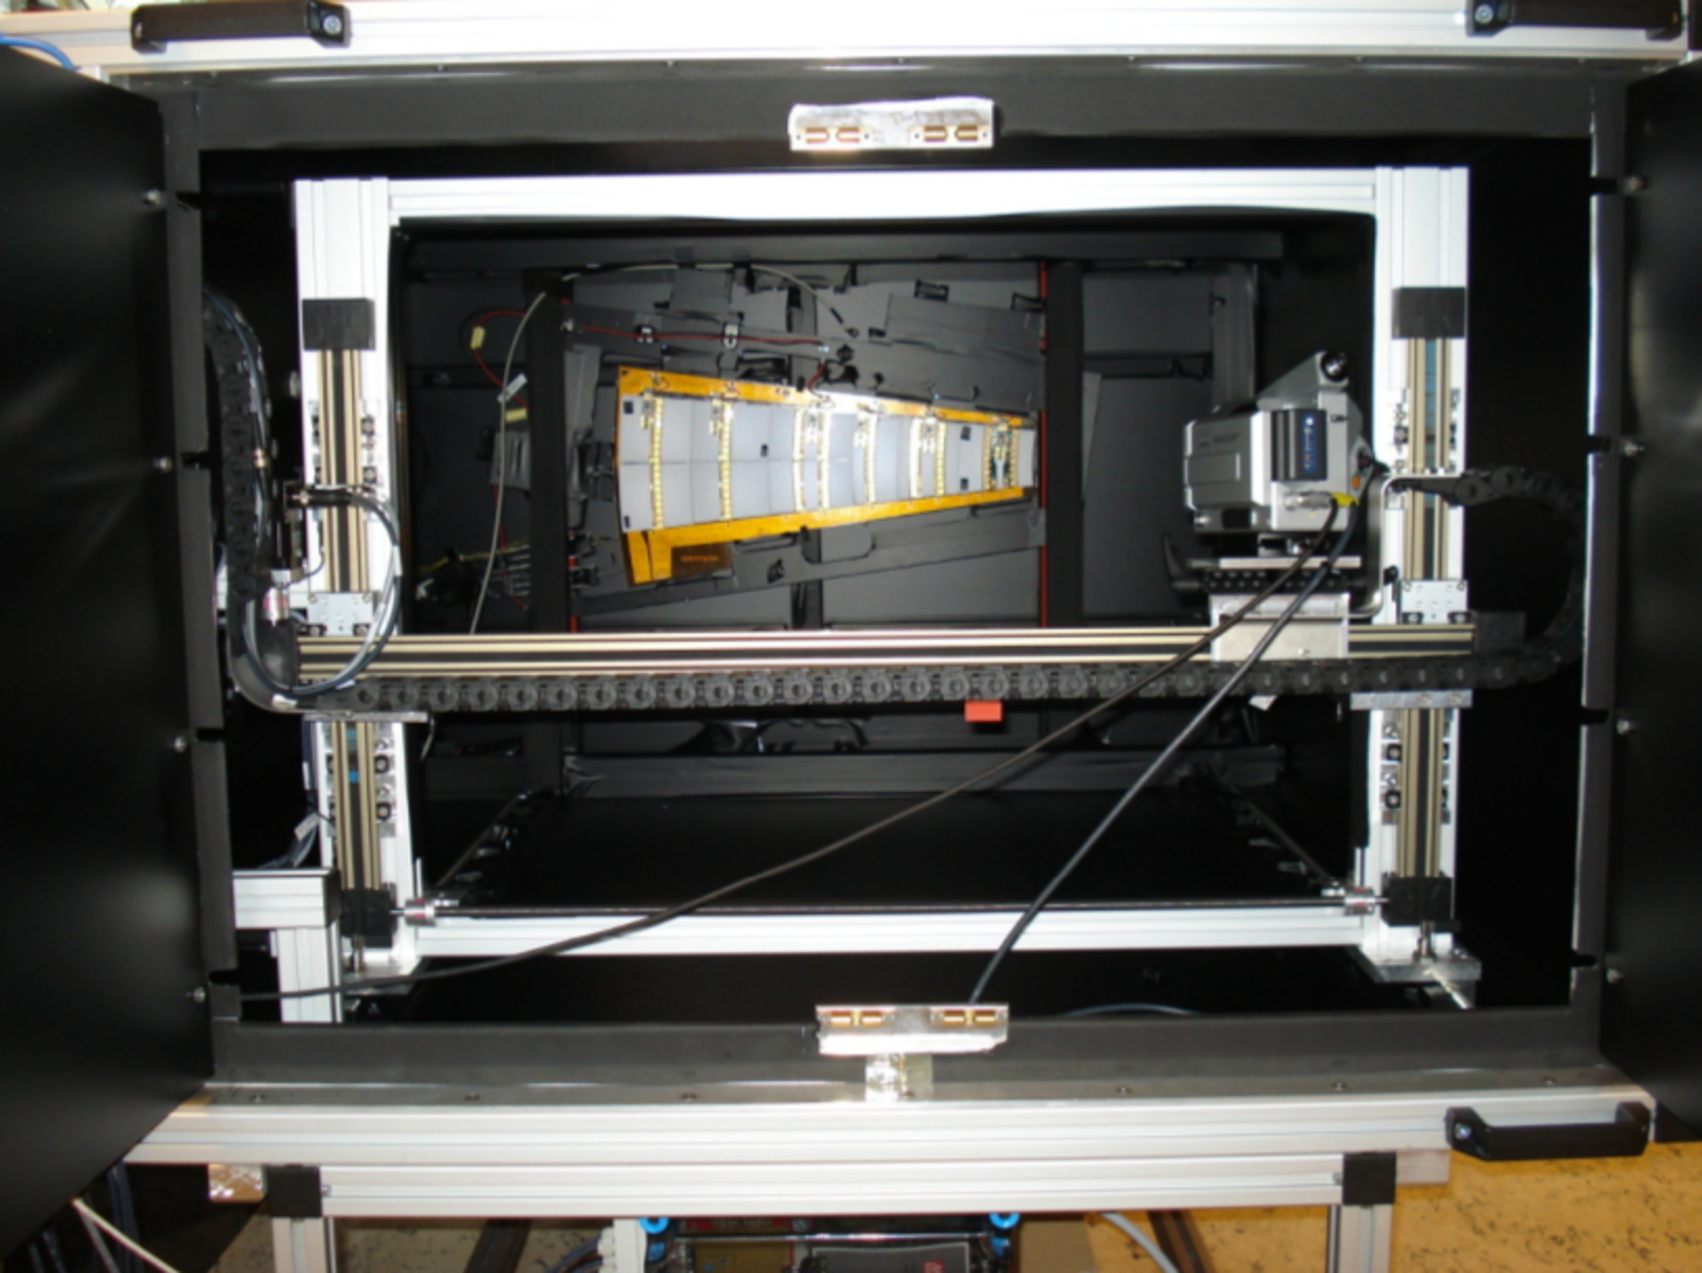
\includegraphics[scale=0.26]{Figures/Chapter02/CamberFront.pdf}
			\caption{Image of both ends of the thermal chamber showing the Petal already in place and the IR camera also in position.}\label{fig5}
		\end{figure}
		
		The use of the chamber has two main advantages: on one hand, it provides shielding for the object under investigation against external heat sources such as ceiling lamps, computers and other electronic devices used in the setup; on the other hand, it is used as an enclosure where we can flush nitrogen in order to reduce the moisture and in doing so also reduce the potential absorption of IR radiation in the air path from the target to the IR camera.
		
	\section{IR camera.}\label{section2.2}
	
		For this study a VarioCAM High Resolution (hr) IR camera from InfraTec GmbH was used (Figure \ref{fig6}). The VarioCAM \textregistered hr is a thermographic system for the long wave infrared spectral range (LWIR) of (7.5 - 14) $\mu$m. The lens images the object scene onto a microbolometer array at a resolution of (640 x 480) pixels. The electrical signal of the detector arrays is further processed by the internal electronics. The electronics contains all the functions necessary for camera operation, such as activation of the microbolometer array, A/D conversion, offset and gain correction, defective pixel treatment, video and PC interfaces [6].
		
		\begin{table}[ht!]
    		\begin{minipage}[b]{0.4\linewidth}
  				\centering
  				\captionsetup{justification=centering, margin=0.5cm}
  				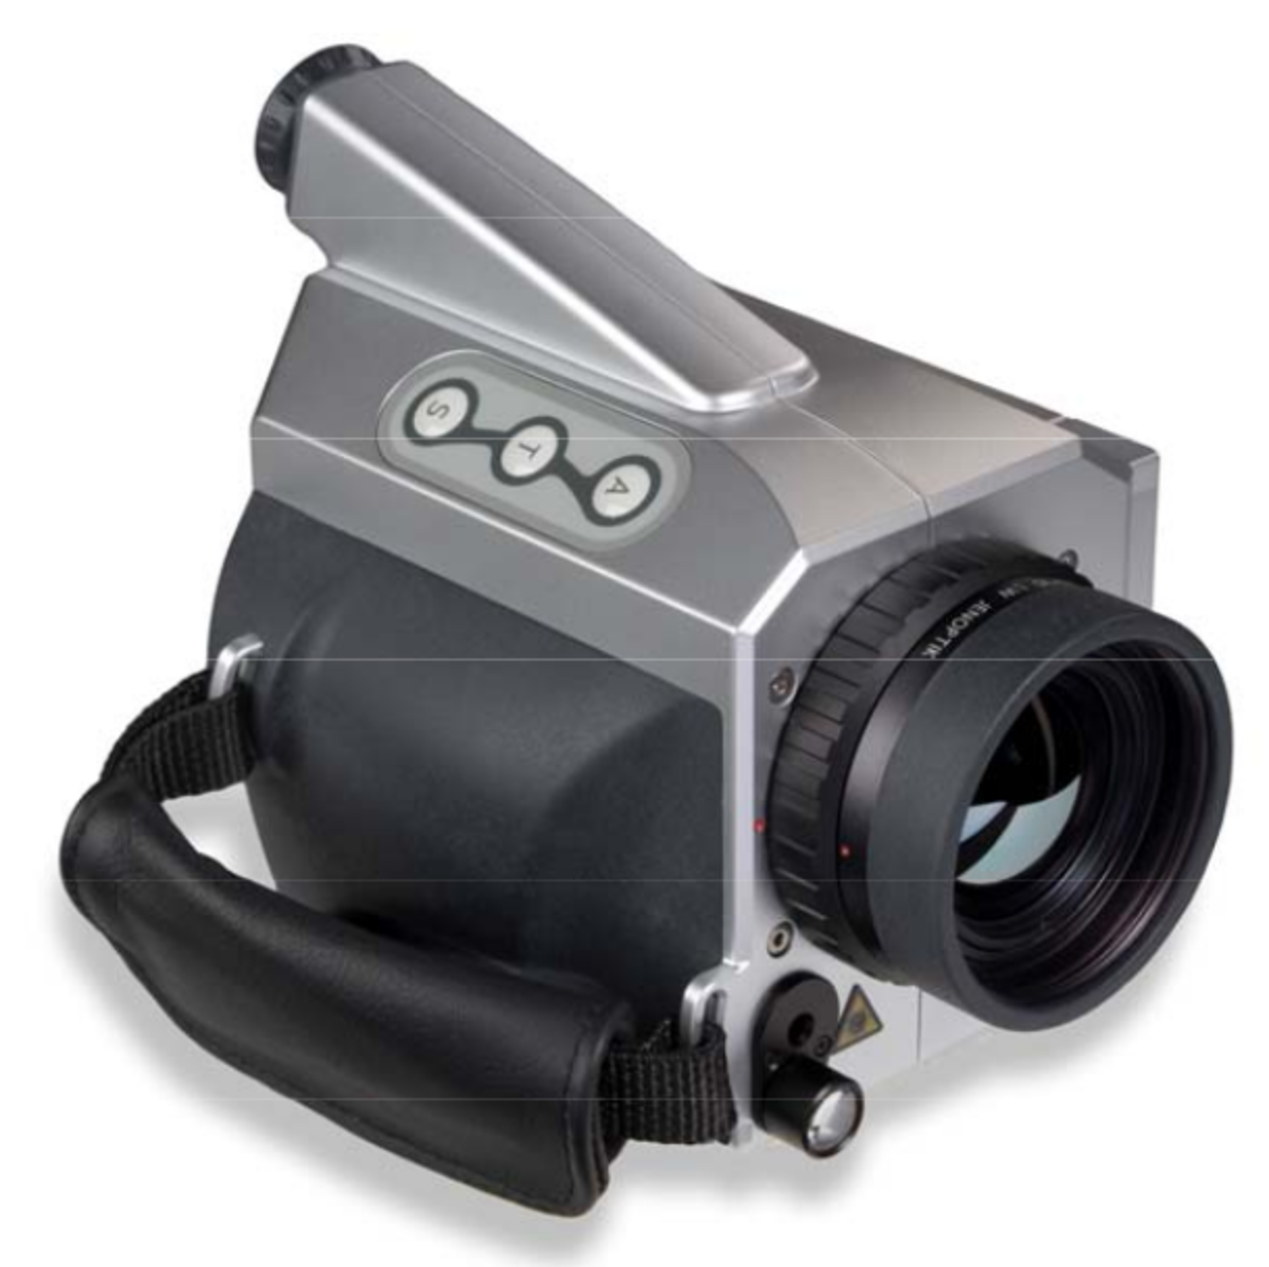
\includegraphics[scale=0.3]{Figures/Chapter02/PictureOfIRCamera.pdf}
  				\captionof{figure}{VarioCAM \textregistered hr (640 x 480 pixels) IR camera  from InfraTec \textcopyright GmbH.}\label{fig6}
    		\end{minipage}
    		\begin{minipage}[b]{0.7\linewidth}
    			\centering
  				\captionsetup{justification=raggedright}
        		\caption{VArioCam hr technical data.}\label{tab1}
				\begin{tabular}{p{0.35\linewidth}p{0.35\linewidth}}\hline
					\textbf{Temperature measuring range} & (-40 ... 1.200) $^{\circ}C$, optional $>$ 2.000 $^{\circ}C$ \\ \hline 
					\textbf{Temperature resolution @ 30 $^{\circ}C$} &  better than 0.08 K, up to 0.05 K (premium mode) \\ \hline
					\textbf{Emissivity} & Adjustable from 0.1 to 1.0, in increments of 0.01 \\ \hline
					\textbf{Detector} &  uncooled microbolometer Focal Plane Array \\ \hline
					\textbf{A/D conversion} &  16 bit \\ \hline 
					\textbf{Operation temperature} & (-15 ... 50) $^{\circ}C$ \\ \hline
					\textbf{Humidity during operation and storage} & 5\% to 95\%, non-condensing \\ \hline
					\textbf{Shock resistance} & 25 G, IEC 68-2-29 \\ \hline
				\end{tabular}
    		\end{minipage}
		\end{table}
		
		The camera's accuracy for temperature measurement (reported by manufacturer) is $\pm$1.5 K in the range from 0 $^{\circ}C$ to 100 $^{\circ}C$ and $\pm$2\% anywhere outside that range. Some additional technical data is presented in Table \ref{tab1}.
		
		The data acquisition is performed using the VarioCam hr control software IRBIS \textregistered professional v3.1 (Figure 2.3). The images are taken in bursts of 100 pics (in approximately 5 seconds) and then averaged in order to reduce uncertainty due to pixels noise. All thermograms are recorded in units of absolute temperature (K) and emissive power ($W/m^2$) for offline analysis.
		
		\begin{figure}[ht!]
			\centering
			\captionsetup{justification=centering,margin=2cm}
			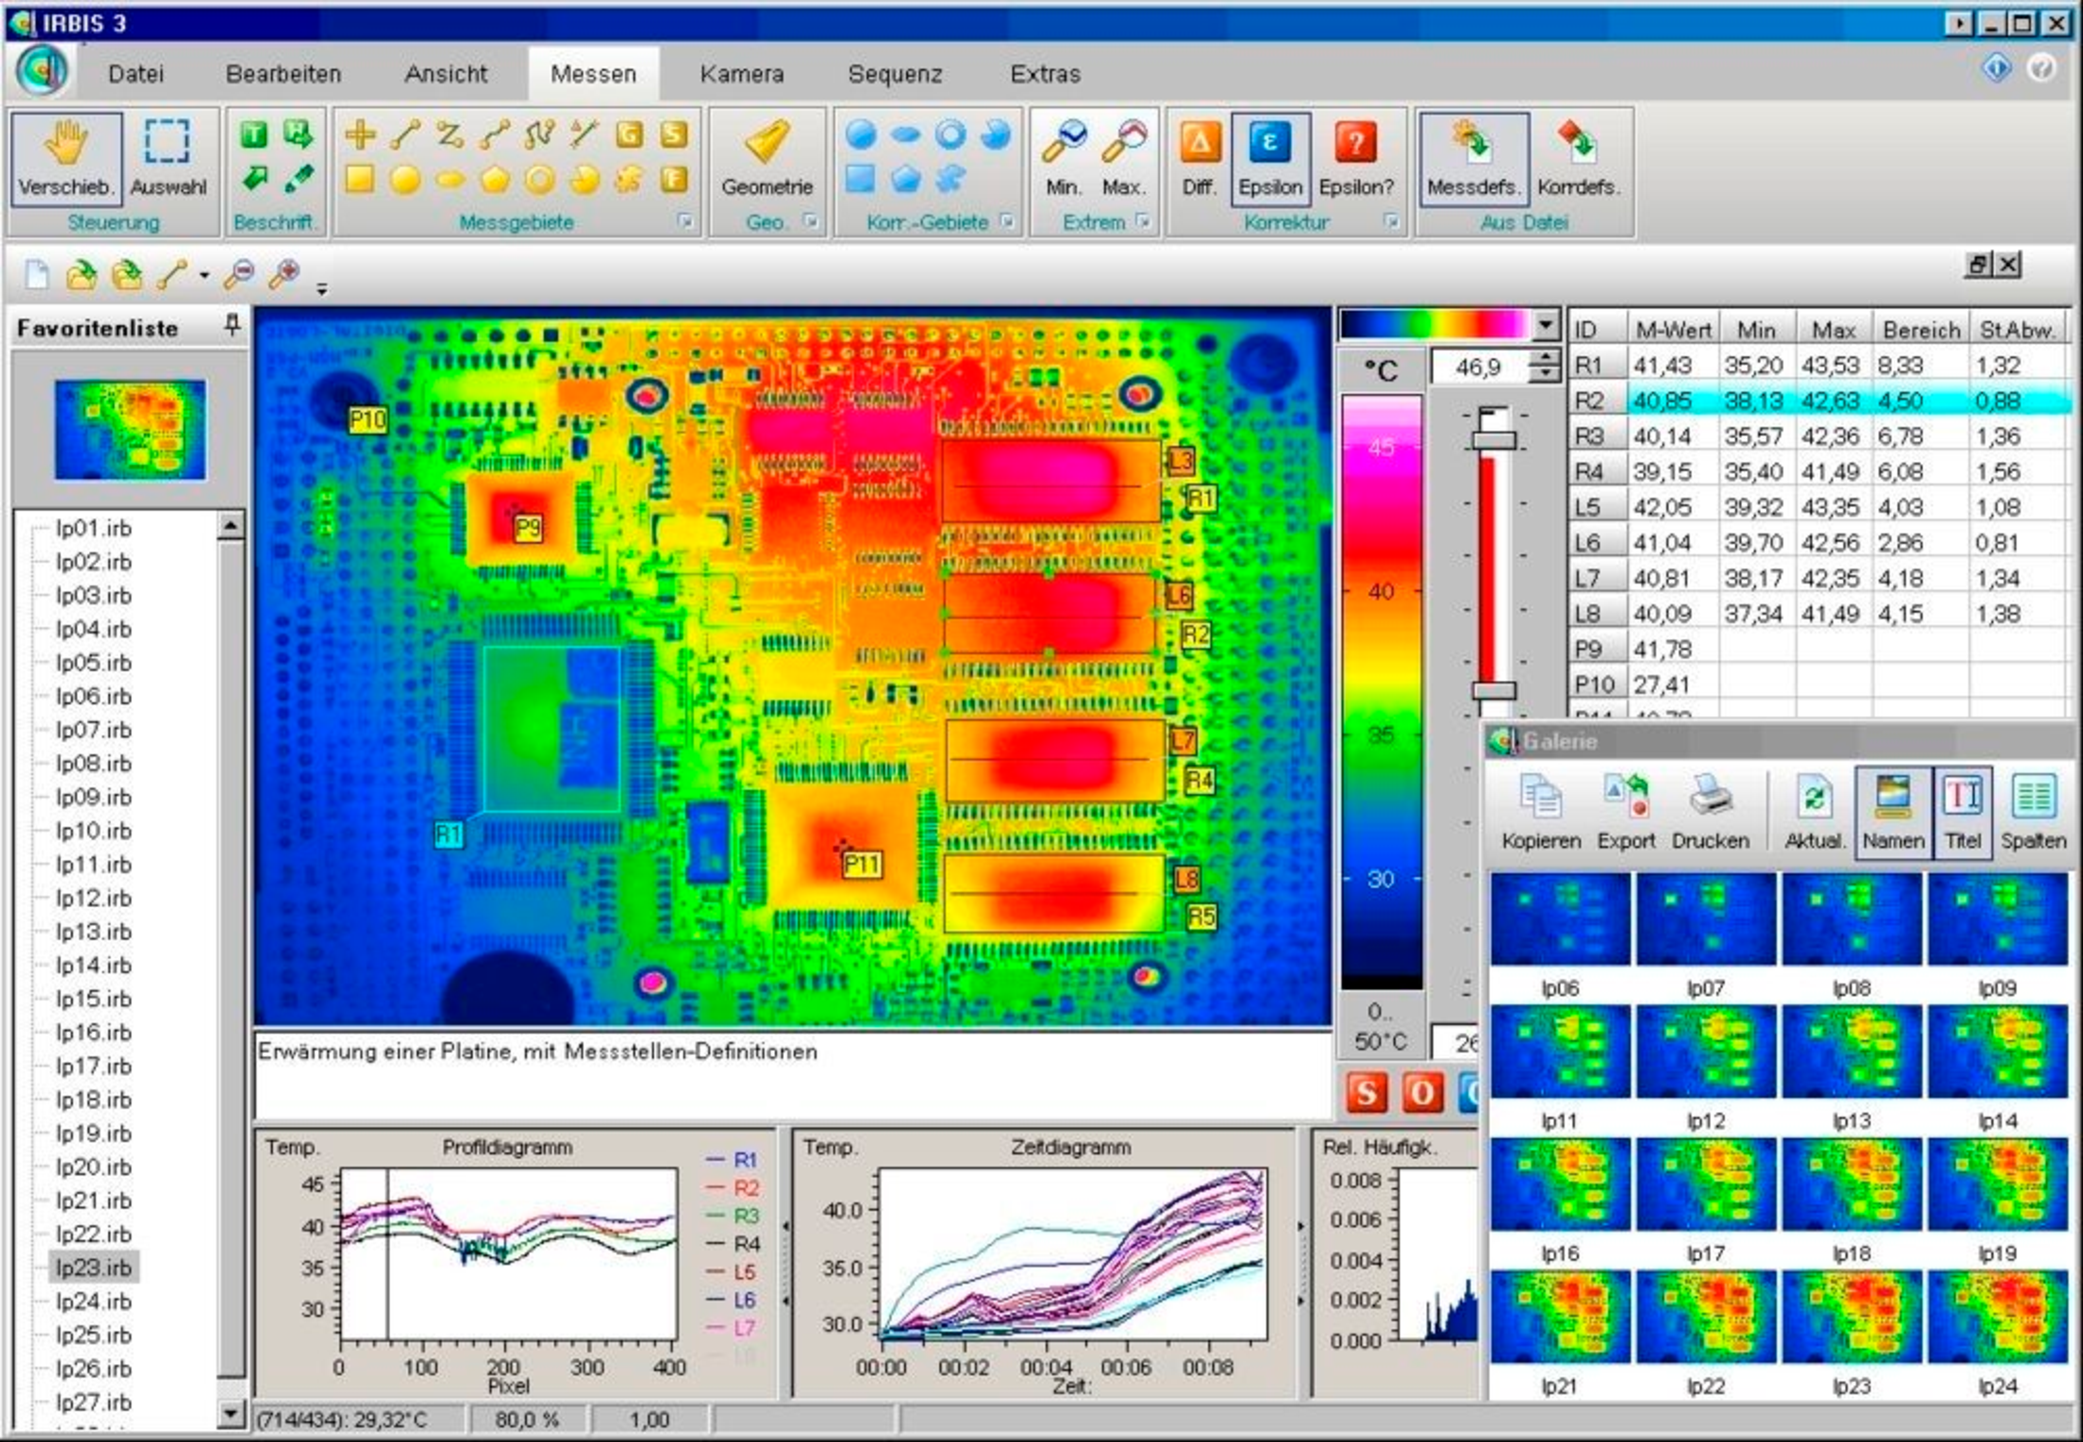
\includegraphics[scale=0.35]{Figures/Chapter02/IRBISimage.pdf}
			\caption{Screenshot of the camera’s control software IRBIS \textregistered 3.1.}\label{fig7}
		\end{figure}

		It is important to point out the fact that the software does not gives us the “real” temperature values but rather an “apparent” one. We refer to this temperatures reported by the IR software as apparent temperatures since it's necessary later on to correct them due to emissivity, reflectivity and other effects that provoque deviations in what the IR sensor perceives as temperature (See Chapter 3).
		
	\section{Thermo Mechanical Petal.}\label{section2.3}
	
		The petal structure is the frame where the end-cap sensors are mounted. It provides the mechanical and electronic structural support and also contains a titanium alloy cooling pipe for evaporative $CO_{2}$ cooling. For the Phase-II ATLAS upgrade new Petal designs are still under development. However, in this study a thermomechanical prototype manually assembled is used, equipped with dummy electronics parts, blank silicon wafers and mechanical components to be a thermal equivalent to the final structure (Figure \ref{fig8}). As the petal's design is still being improved, our prototype became quickly “obsolete”. In fact, some key materials for IR studies in the current prototype such as the silicon wafers are not very IR friendly because of their high transmissivity. This makes really difficult the employment of non-contact temperature measuring methods (See Chapter 3). In contrast, newer silicon wafers are available which are not transmissive due to a metallic finish in one of their sides, in that cases, even though the emissivity of silicon is hard to estimate, more robust IR studies can be performed.
		
		\begin{figure}[ht!]
			\centering
			\captionsetup{justification=centering,margin=2cm}
			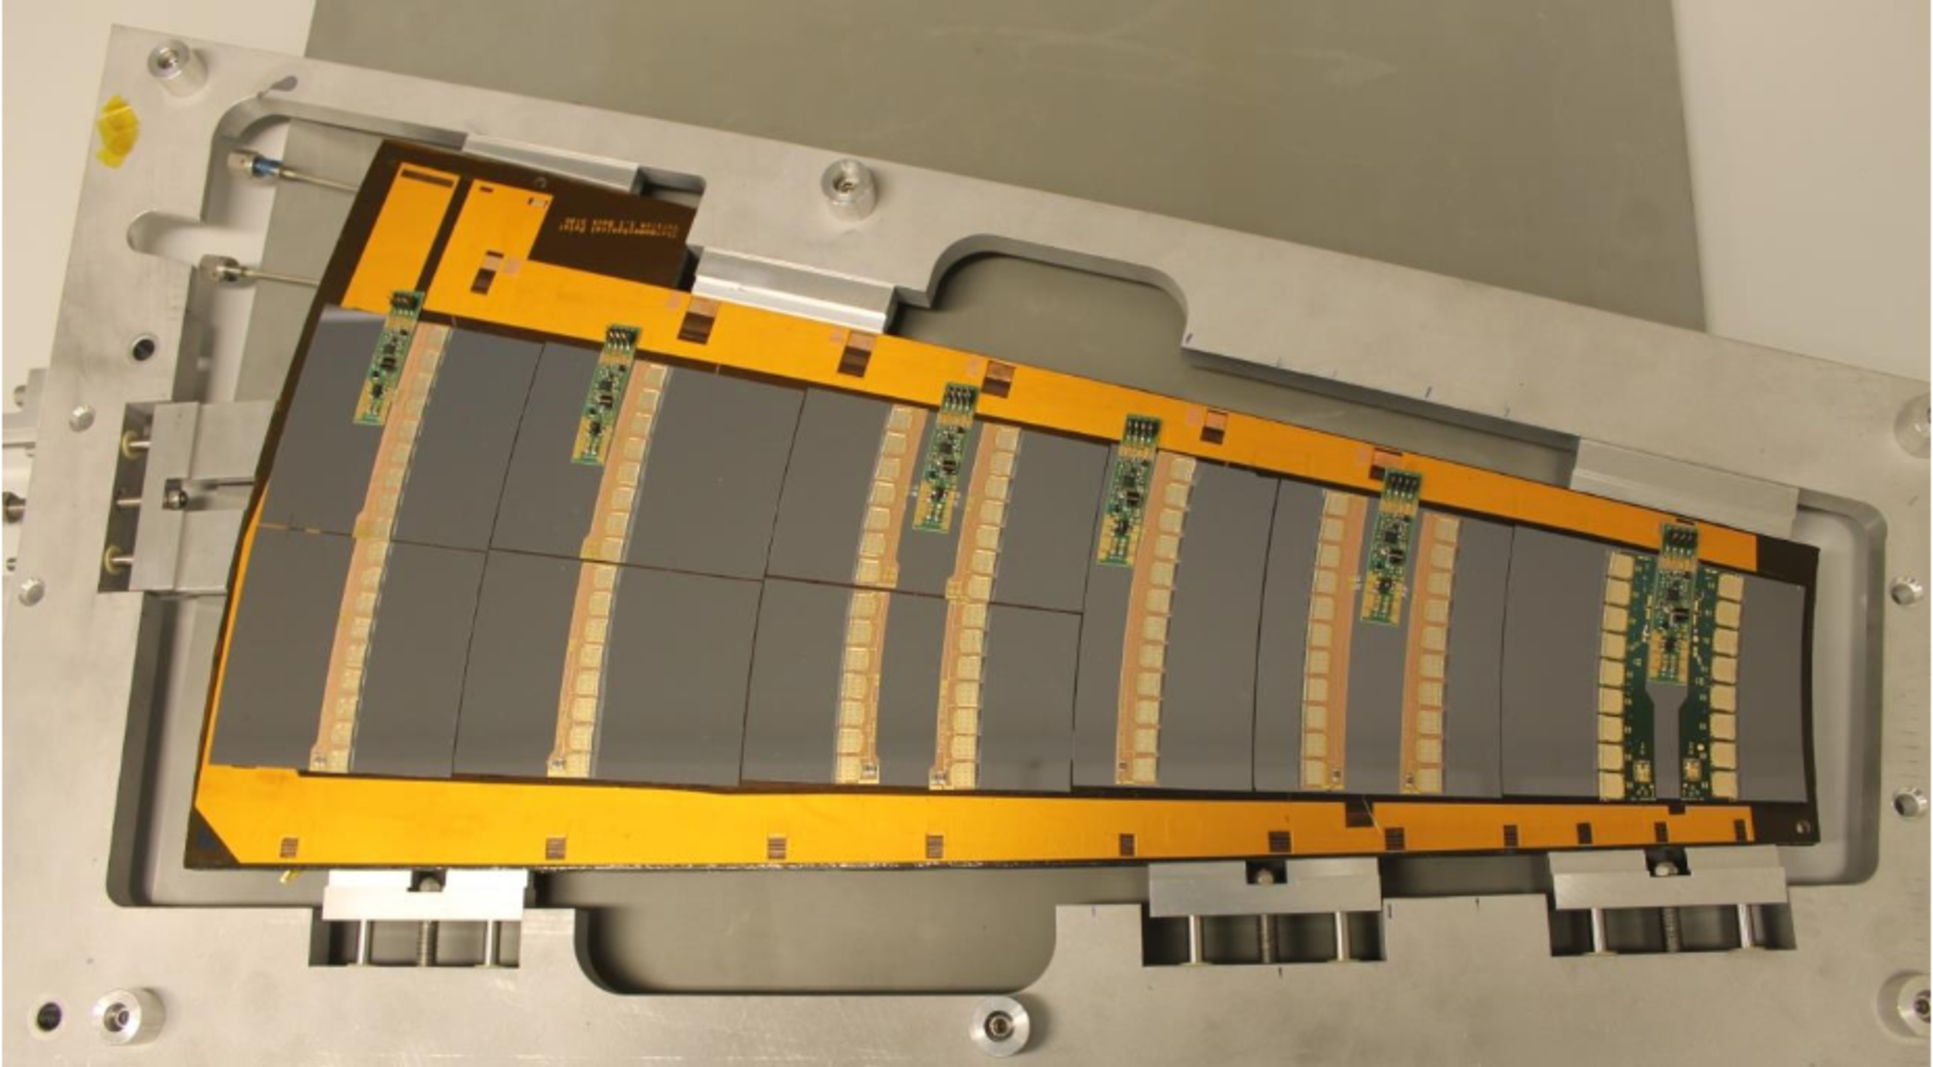
\includegraphics[scale=0.35]{Figures/Chapter02/PetalConstruction.pdf}
			\caption{Thermomechanical prototype of the Petal used in the IR measurements.}\label{fig8}
		\end{figure}
		
		The petal prototype is composed by 6 modules named R0 (closest to the beamline in the radial direction), R1, R2, R3, R4 and R5 (Figure \ref{fig9}). Each module contains, in general, the following components:
		
		\begin{itemize}
			\renewcommand{\labelitemi}{$\diamond$}
			\item Blank Si, laser cut (320 $\mu$m thick).
			\item FR4 PCBs (200 $\mu$m thick).
			\item Glass ASICs with heater pattern and bonding pads, glued with UV glue, wire-bonded to bare silicon.
			\item Real DC-DC converters, based on commercial LTC360 ASIC on a custom board.
			\item Potentiometer to adjust power input/output.
			\begin{itemize}
			\renewcommand{\labelitemi}{$\bullet$}
				\item Powered through bus tape power lines.
			\end{itemize}
			\item In the case of R0 module: v0 assembly tools, real hybrids, glass ASICs.
		\end{itemize}
		
		In addition, the prototype counts with real cores, real copper power traces, dummy data-lines, dummy EoS (not present initially but recently installed) and a 1.5 mm diameter titanium cooling pipe.
		
		\begin{figure}[ht!]
			\centering
			\captionsetup{justification=centering,margin=2cm}
			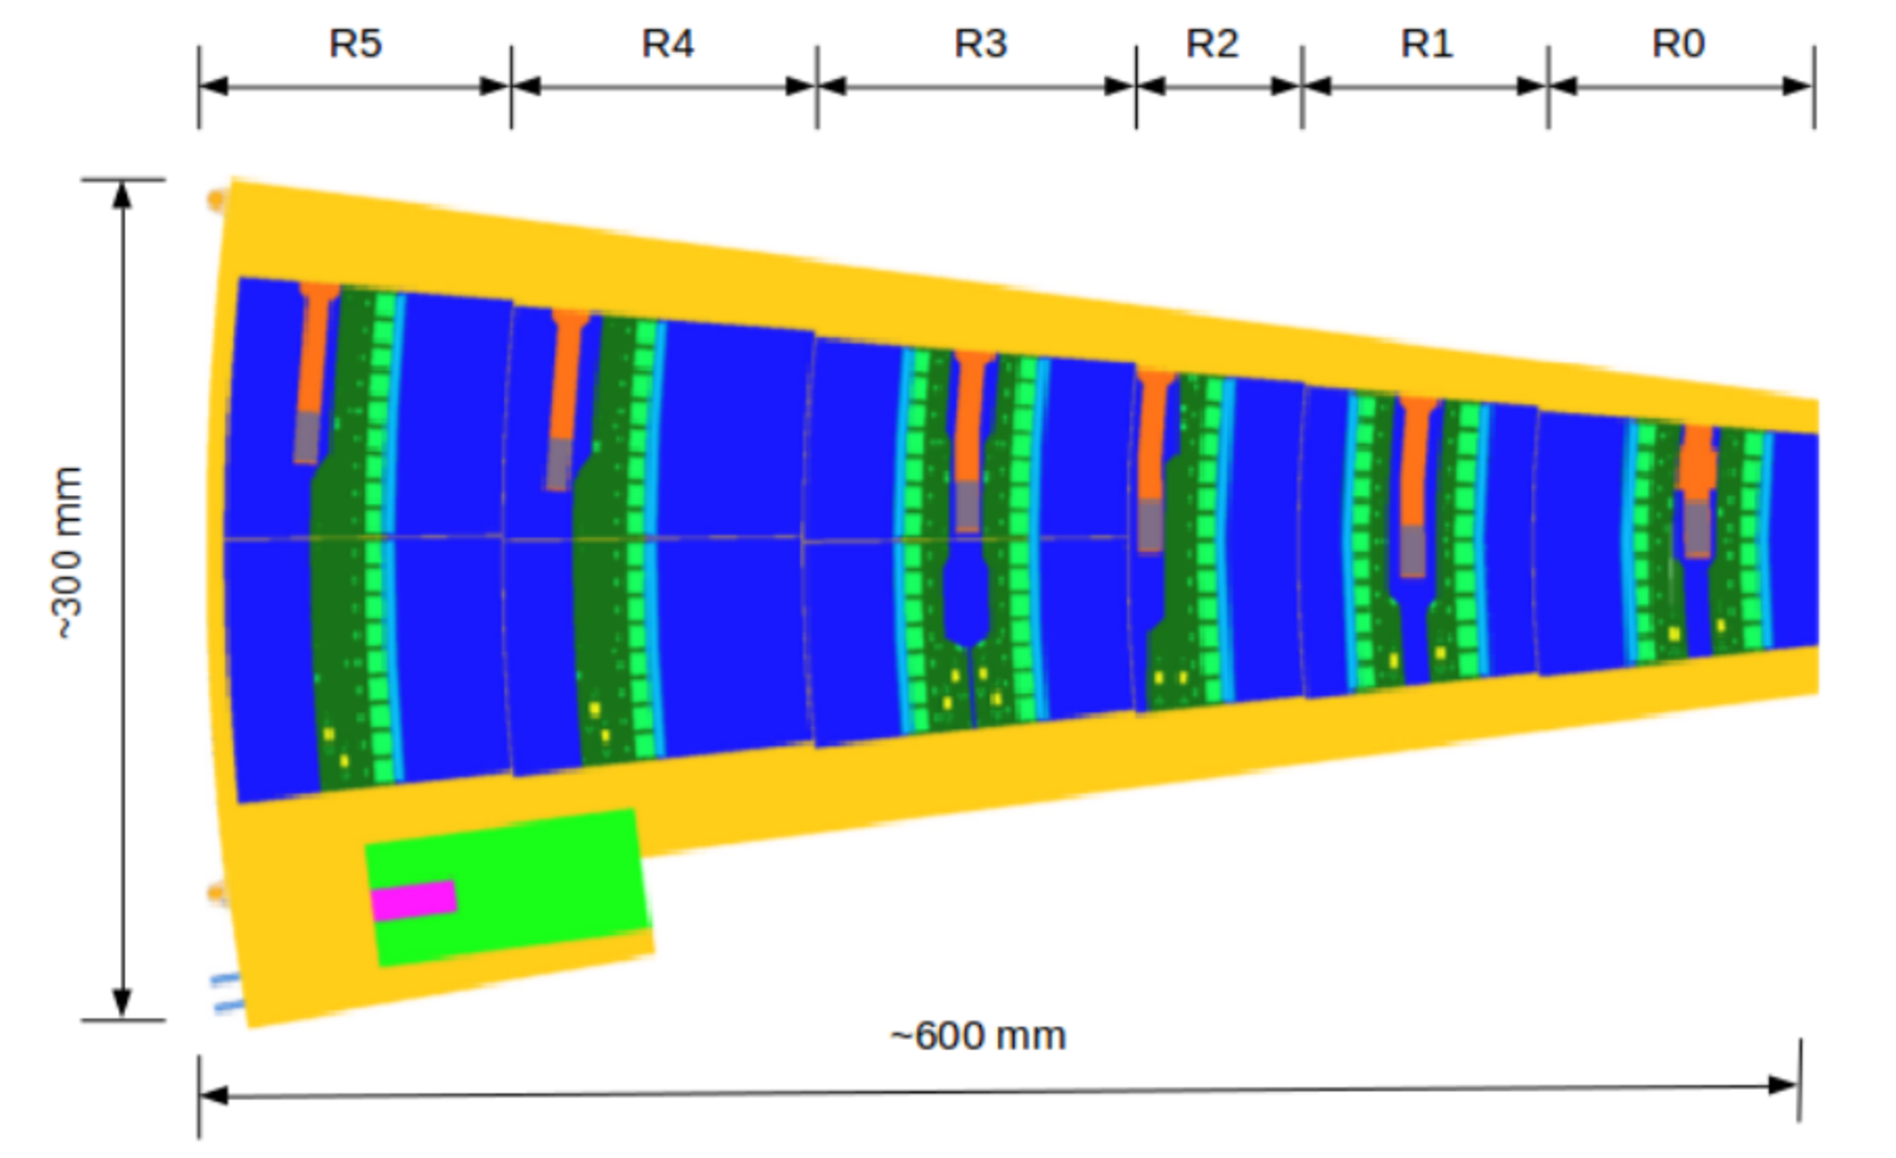
\includegraphics[scale=0.35]{Figures/Chapter02/PetalDesign.pdf}
			\caption{Design of the petal showing the 6 different modules.}\label{fig9}
		\end{figure}
		
	\section{Setup configuration.}\label{section2.4}
	
		In this study the results of two thermal cycles performed using the setup described below are considered, corresponding to both sides of the Petal and measured with the latest experimental configuration. In the following, this will be referred to as “cycle 2” (unpolished side) and “cycle 9” (polished side) in allusion to the dates in which the measurements began (August 2nd and August 9th, 2017). 
		In order to perform the IR measurements, the TM Petal prototype is placed in the thermal chamber as shown in Figure \ref{fig5} (left) and the IR camera is positioned in such a way that it faces the Petal with an angle (Figure \ref{fig10}). This is done in order to avoid the Narcissus effect which is basically the heat from the camera itself being reflected back and measured.
		As mentioned before, nitrogen is flushed into the chamber to reduce the moisture and avoid the appearance of ice that could destroy the Petal. Also, this prevents condensation, which is particularly dangerous in the electronic components of the prototype.
		
		\begin{figure}[ht!]
			\centering
			\captionsetup{justification=centering,margin=2cm}
			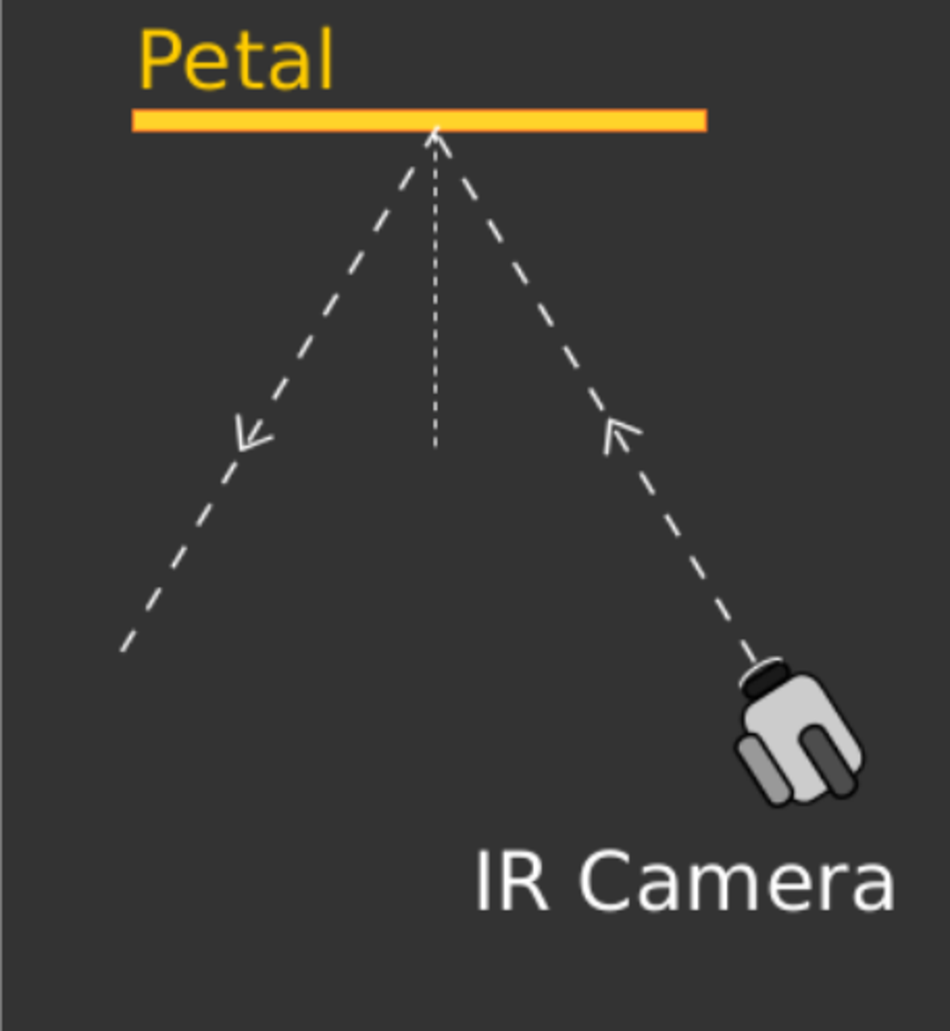
\includegraphics[scale=0.35]{Figures/Chapter02/NarcissusEffect.pdf}
			\caption{The IR camera is placed at some angle with respect to the plane of the petal to avoid Narcissus effect.}\label{fig10}
		\end{figure}
		
		Further improvements came from experiences of preliminary tests when we realized that, for example, the heat from the Gantry system was being reflected on the Petal's surface and registered by the IR camera. Then, a curtain from an opaque black fabric was placed between the Petal and the Gantry system (leaving a small gap for the camera lens) to suppress this effect (Figure \ref{fig11} right). In addition, other improvements to the chamber's insulation were made to better control the ambient conditions inside at lower temperatures and also to avoid the loss of nitrogen during the tests (Figure \ref{fig11} left). This is particularly important for an accurate estimation of the apparent reflected temperature (See section 3.1.1). In addition, the DC-DC converters in modules R2 and R3 were covered with 3D-printed caps and black tape due to the fact that their heat created a “halo” of hot air around them that strongly interfered with the IR measurements of that area of the Petal (Figure \ref{fig12} left).
		
		\begin{figure}[ht!]
			\centering
			\captionsetup{justification=centering,margin=2cm}
			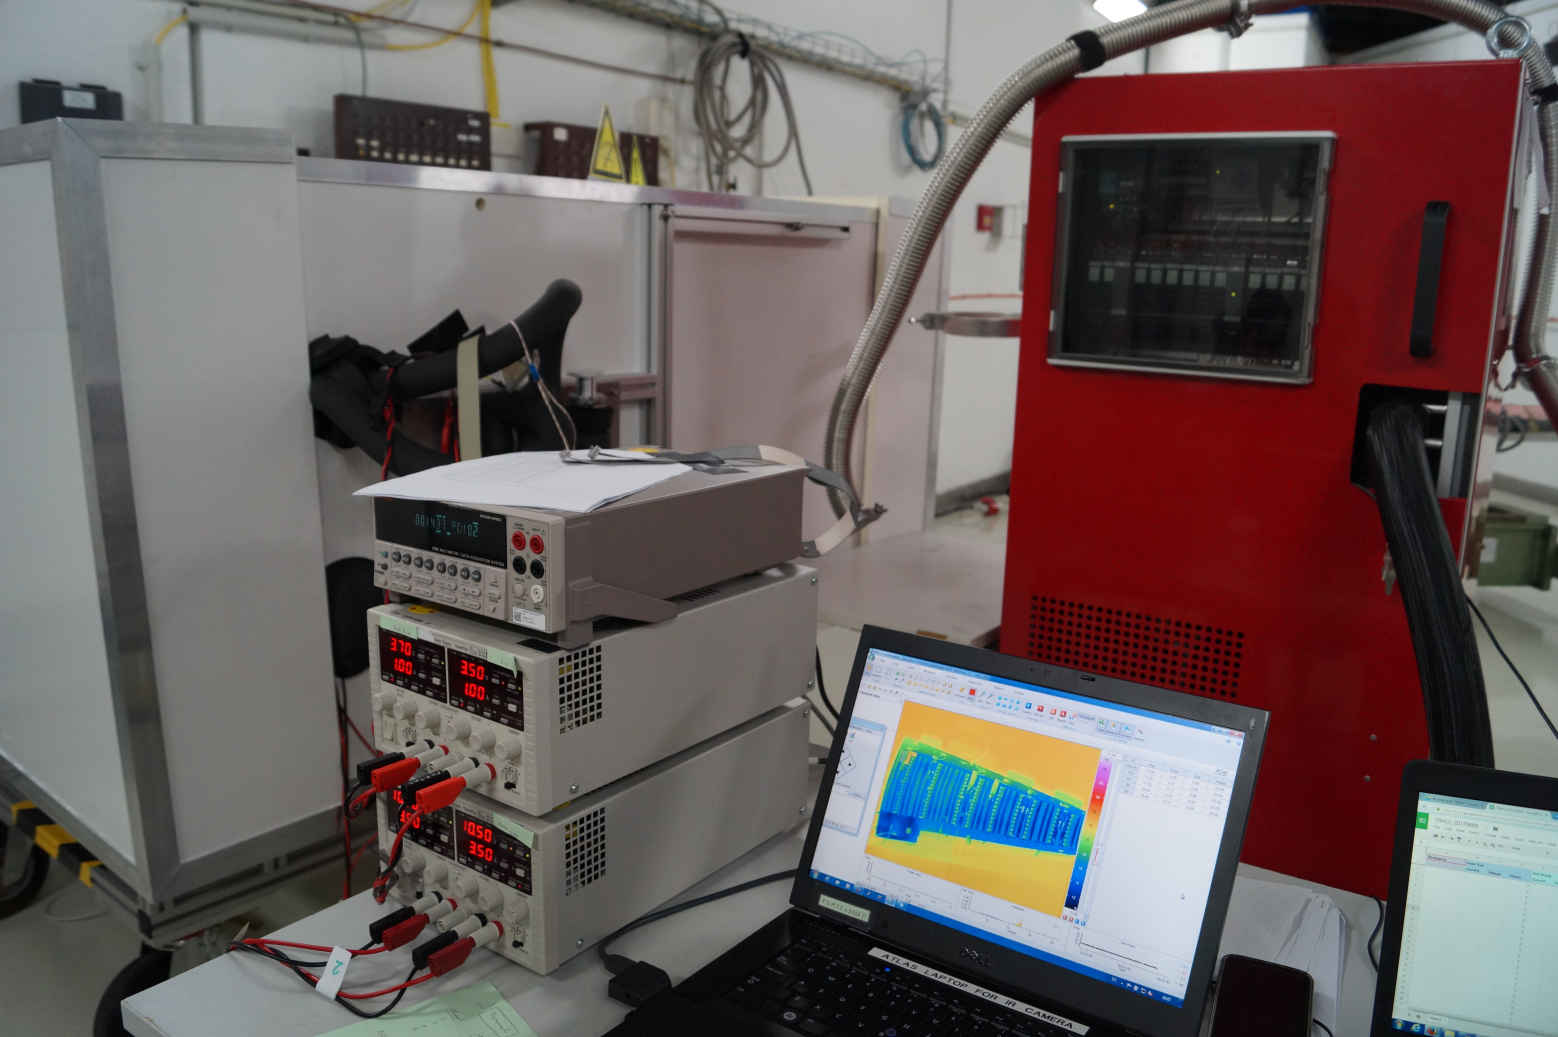
\includegraphics[scale=0.18]{Figures/Chapter02/ExperimentalSetup.pdf}
			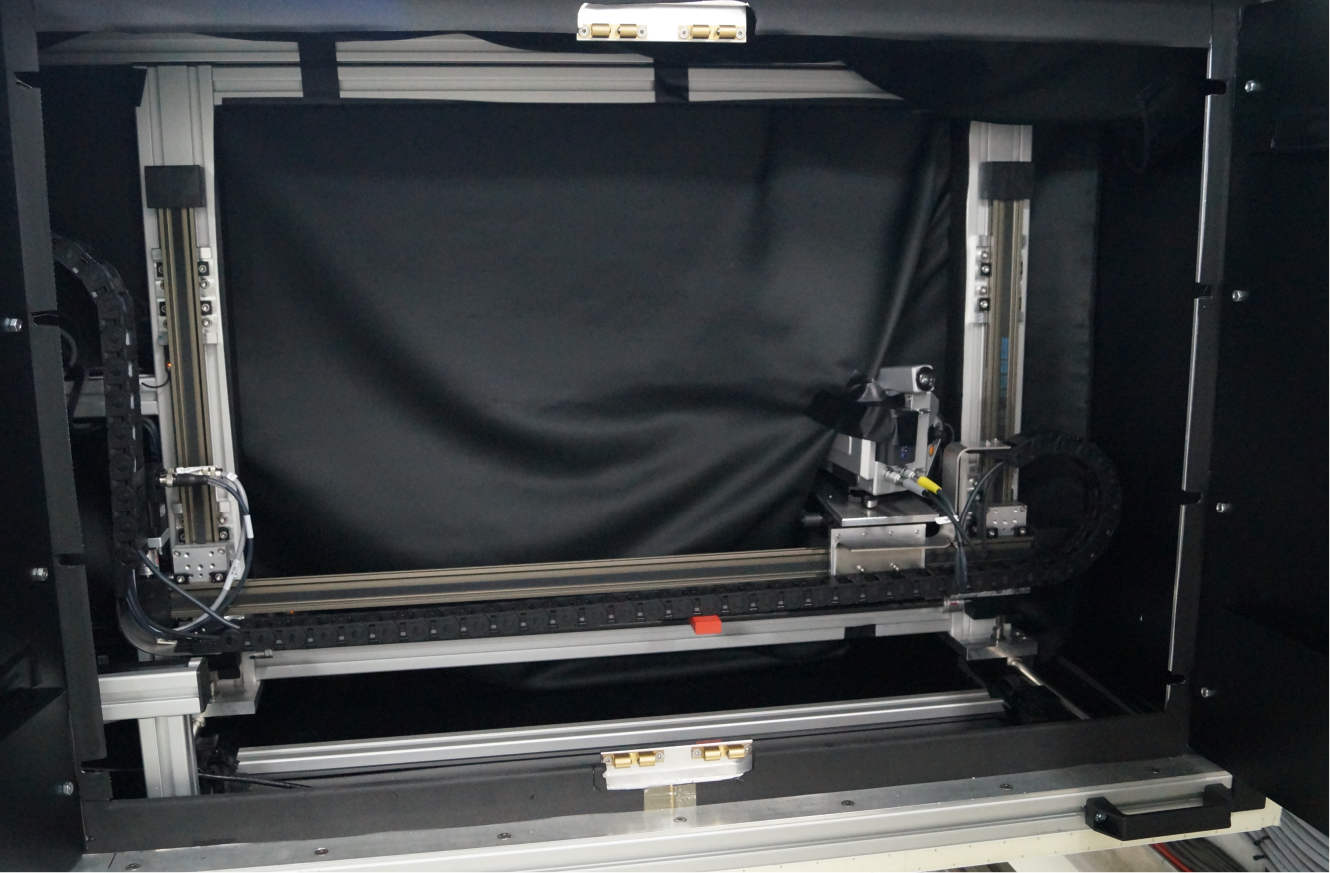
\includegraphics[scale=0.215]{Figures/Chapter02/BlackCurtine.pdf}
			\caption{Experimental setup used for the Petal's thermal cycles.}\label{fig11}
		\end{figure}
		
		For cooling the Petal the Transportable Refrigeration Apparatus for $CO_{2}$ Investigation (TRACI) was used (Red box in Figure \ref{fig11} left). By controlling the $CO_{2}$ pressure in the experiment we were able to adjust the desired temperature working point. Using this method temperatures of near -25 $^{\circ}C$ were reached. Table \ref{tab2} shows the nominal temperature output of the $CO_{2}$ for any given pressure set point.
		
		\begin{table}[ht!]
			\captionsetup{justification=raggedright}
        	\caption{Relation between pressure and temperature for $CO_{2}$.}\label{tab2}
        	\centering
			\begin{tabular}{||P{0.14\linewidth}|P{0.14\linewidth}||P{0.14\linewidth}|P{0.14\linewidth}||P{0.14\linewidth}|P{0.14\linewidth}||} \hline\hline
				\textbf{Pressure (bar)} & \textbf{Temperature ($^{\circ}C$)} & \textbf{Pressure (bar) (cont.)} & \textbf{Temperature ($^{\circ}C$) (cont.)} & \textbf{Pressure (bar) (cont.)} & \textbf{Temperature ($^{\circ}C$) (cont.)} \\ \hline\hline
				10 & -40.1 & 27 & -9.3 & 44 &  9.1 \\
				11 & -37.5 & 28 & -8.0 & 45 & 10.0 \\
				12 & -35.1 & 29 & -6.8 & 46 & 10.9 \\ 
				13 & -32.8 & 30 & -5.6 & 47 & 11.7 \\
				14 & -30.6 & 31 & -4.4 & 48 & 12.6 \\
				15 & -28.5 & 32 & -3.2 & 49 & 13.5 \\
				16 & -26.6 & 33 & -2.0 & 50 & 14.3 \\
				17 & -24.7 & 34 & -0.9 & 51 & 15.1 \\
				18 & -22.9 & 35 &  0.2 & 52 & 15.9 \\
				19 & -21.2 & 36 &  1.2 & 53 & 16.7 \\
				20 & -19.5 & 37 &  2.3 & 54 & 17.5 \\
				21 & -17.9 & 38 &  3.3 & 55 & 18.3 \\
				22 & -16.4 & 39 &  4.3 & 56 & 19.0 \\
				23 & -14.9 & 40 &  5.3 & 57 & 19.8 \\
				24 & -13.4 & 41 &  6.3 & 58 & 20.5 \\
				25 & -12.0 & 42 &  7.2 & 59 & 21.3 \\
				26 & -10.7 & 43 &  8.2 & 60 & 22.0 \\ \hline\hline
			\end{tabular}
		\end{table}
		
		Finally, to power each side of the Petal and both EoS, two TTI CPX400 power supply modules were used and a Keithley 2700 multimeter was employed to measure additional PT100 thermocouples using 4 wire sensing and some other important TRACI parameters like $CO_{2}$ flow. The additional thermocouples were placed as follows (for cycle 2): 2 on the inlet/outlet pipes (glued), 2 in R3 module silicon surface (not glued): 1 between the ASICs and 1 in the corner next to R4 (Figure \ref{fig12} right). For cycle 9 four extra thermocouples were placed in R0, R1, R4 and R5 as shown in Figure \ref{fig13}.
		
		\begin{figure}[H]
		
			\centering
			\captionsetup{justification=centering,margin=2cm}
			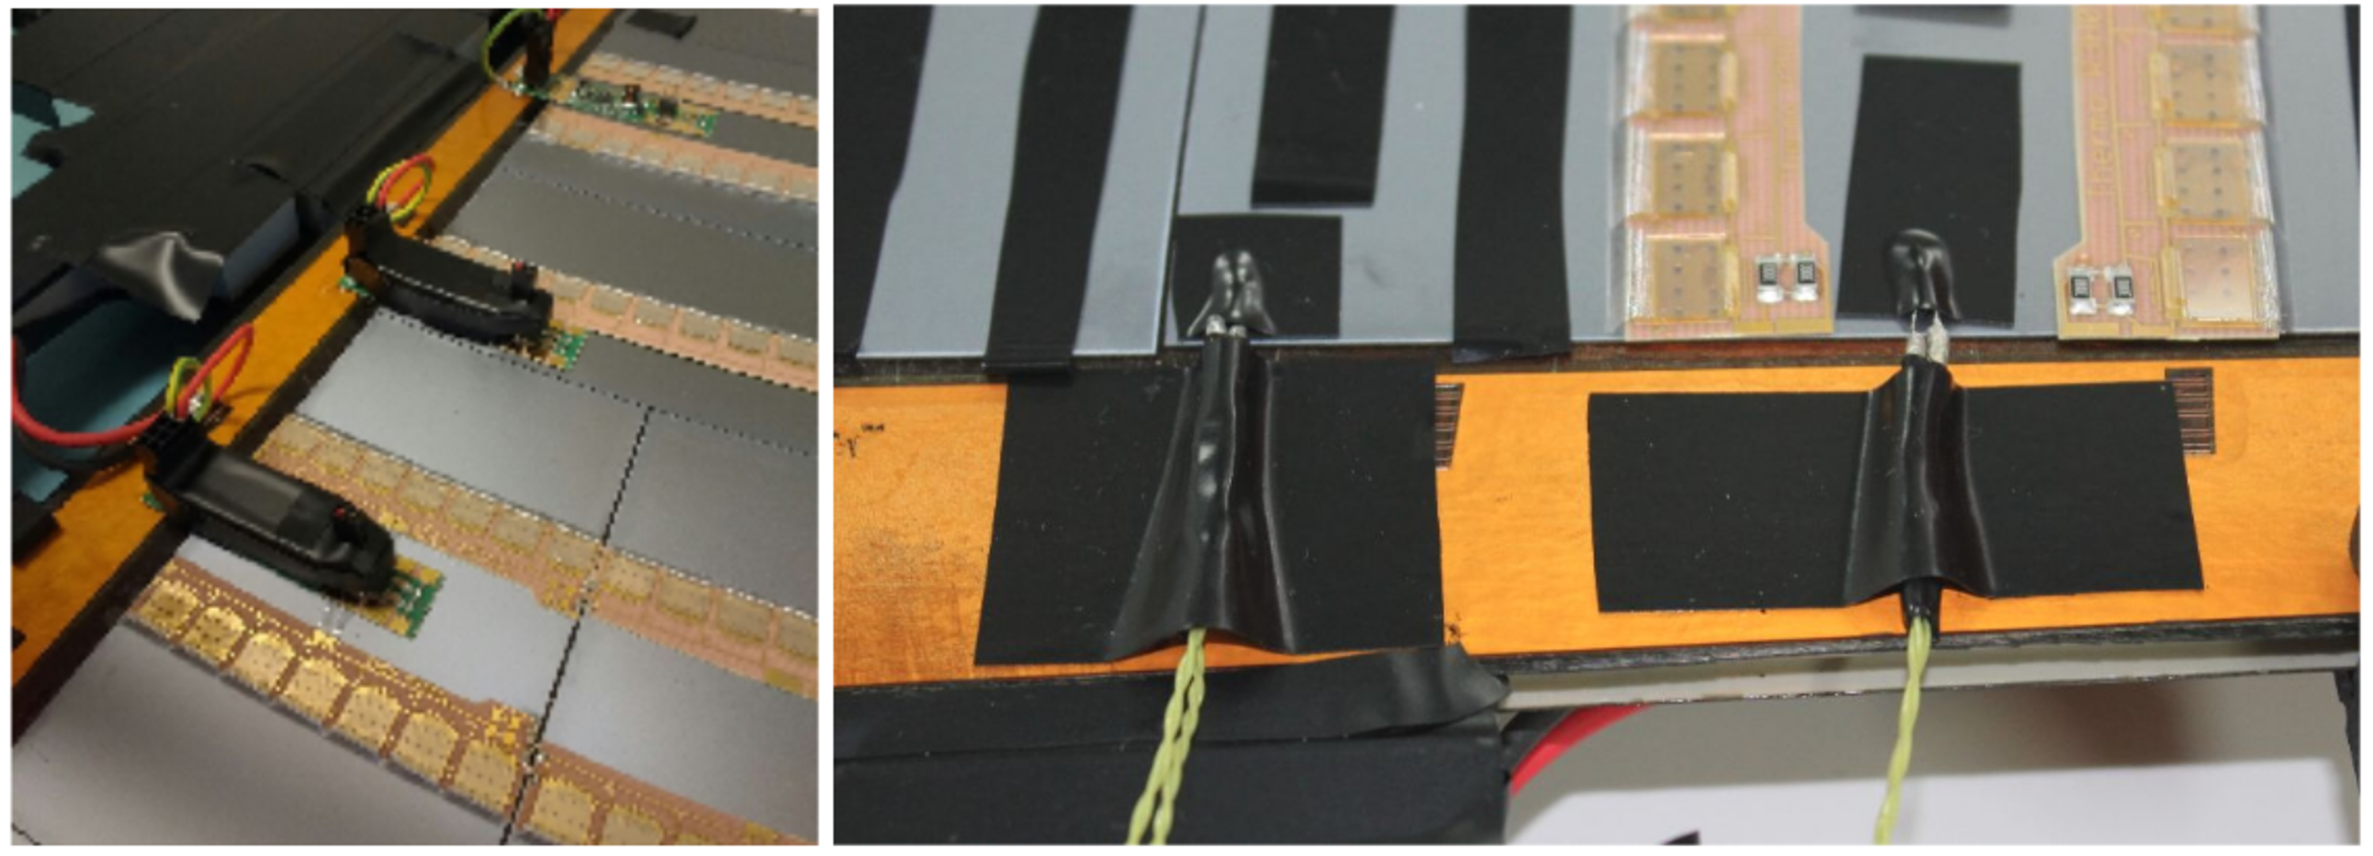
\includegraphics[scale=0.35]{Figures/Chapter02/CloseUpOnTheDCDCcapAndPT100.pdf}
			\caption{Unpolished side of the Petal showing the DC-DC covers (left) and the 2 additional thermocouples attached to R3 module (right).}\label{fig12}
		\end{figure}
		
		\begin{figure}[H]
			\centering
			\captionsetup{justification=centering,margin=2cm}
			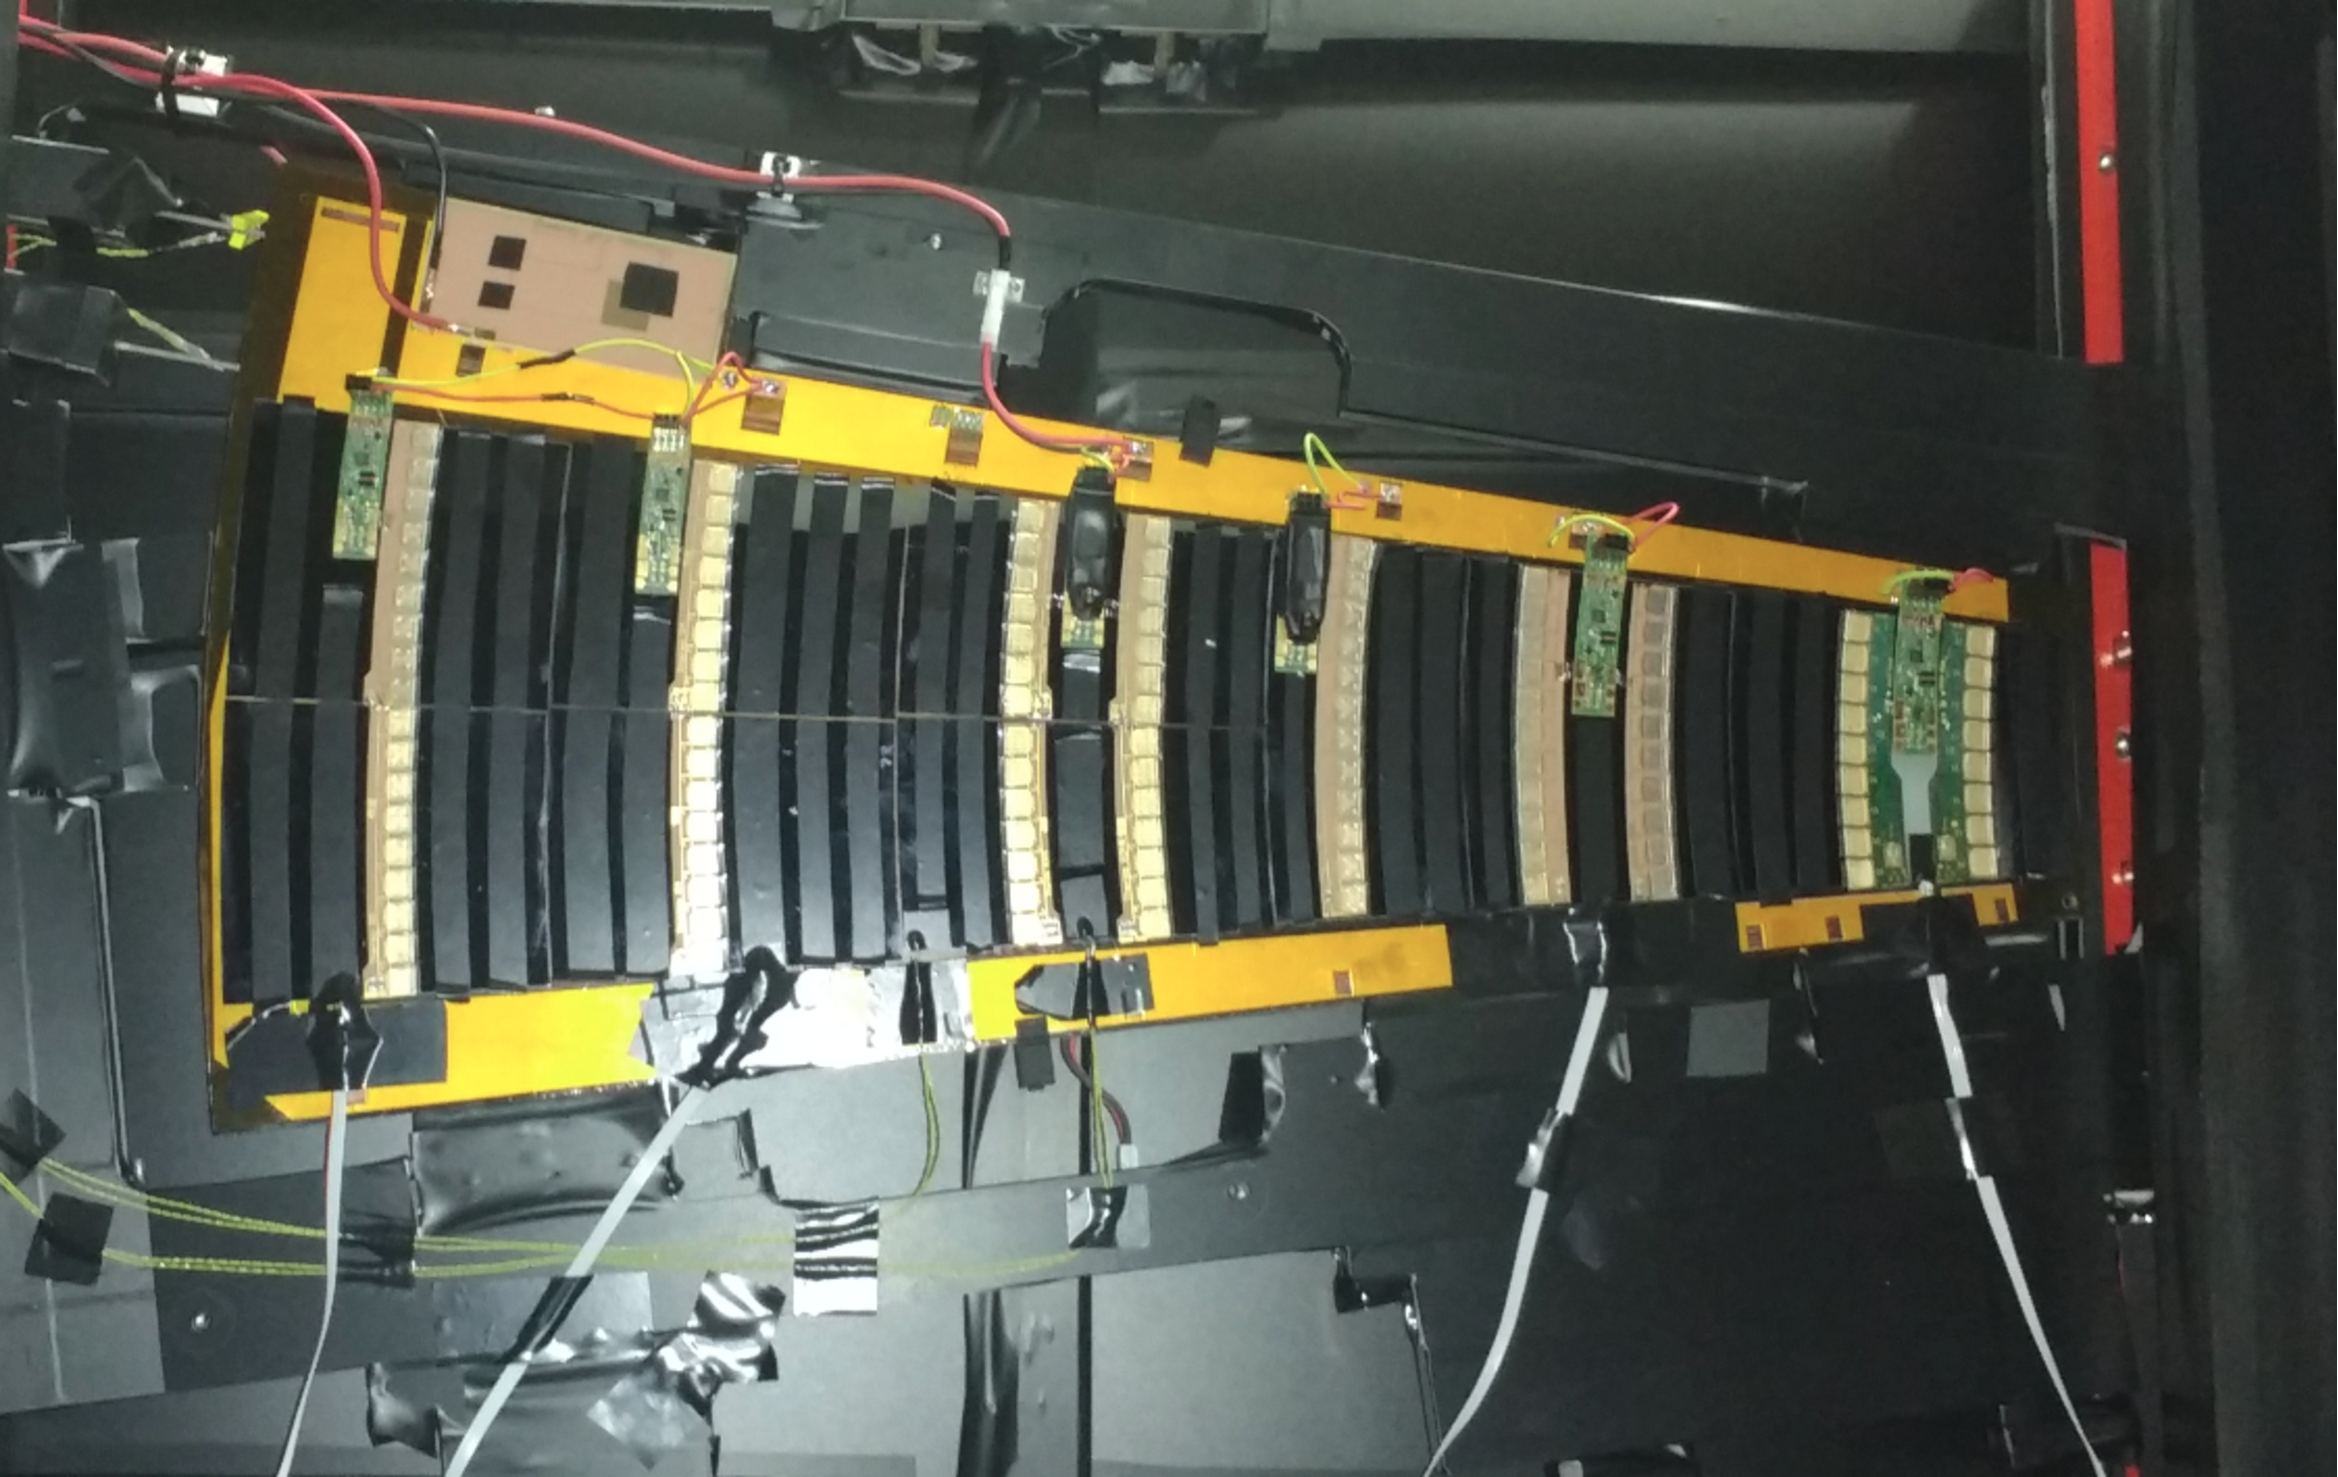
\includegraphics[scale=0.3]{Figures/Chapter02/petal_polished_in_chamber_zoomed.pdf}
			\caption{Polished side of the Petal ready for the thermal test. The additional PT100 thermocouples placed at each module (except R2) are visible (white cables).}\label{fig13}
		\end{figure}

		
